\chapter{Parallel implementation}
In this chapter, we will explain the technical details of the parallel implementation.
First, we will introduce the used technologies/techniques and libraries.
Then we will take a detailed look at the parallelization.


\section{Parallelization techniques}
\subsection{MPI - Message Passing Interface}
MPI (Message Passing Interface) is a standard for a library interface for parallel programs.
MPI is process-based, which means the interface provides a standard to send a message from one process to another process.
The processes can be running on the same machine or on distributed systems like multi-computers or clusters.

If the processes are running on the same machine, MPI does not support shared memory. 
Sending a message from one process to another on the same machine, is a copy operation in the RAM, because the processes have no access to the virtual memory of the other processes.

If the processes are running on distributed systems, MPI sends the messages using the network.
Common networking communications standards are InfiniBand used in high performance clusters, or ethernet and TCP/IP used for the internet.

Messages that can be sent with MPI are sequential arrays of standard data types like integer, floating-point numbers, or characters.
Also, more complex data types can be defined. 
In this work, we send sequential arrays of the type floating-point number.
\newpage
MPI provides many functions to send data.
In this work, we will use the following functions:
\begin{itemize}
	\item MPI\_Bcast: This function broadcasts a sequential array from one process to all other processes. After applying this function, the content of the array is the same on every processor.
	\begin{figure}[H]
		\centering
		\tikzset{
	main/.style={black, line width=0.4mm, opacity=1},
	second/.style={gray, opacity=5},
	arrow/.style={-latex, shorten >=1ex, shorten <=1ex, bend angle=45}
}
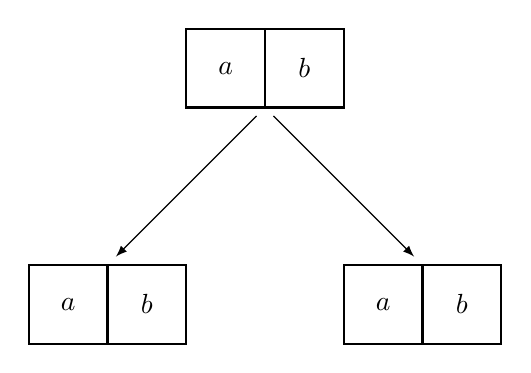
\begin{tikzpicture}

\node (rect) at (2,0) [draw,thick,minimum width=1cm,minimum height=1cm]  {$a$};
\node (rect) at (3,0) [draw,thick,minimum width=1cm,minimum height=1cm]  {$b$};

\node (rect) at (0,-3) [draw,thick,minimum width=1cm,minimum height=1cm] {$a$};
\node (rect) at (1,-3) [draw,thick,minimum width=1cm,minimum height=1cm] {$b$};

\node (rect) at (4,-3) [draw,thick,minimum width=1cm,minimum height=1cm] {$a$};
\node (rect) at (5,-3) [draw,thick,minimum width=1cm,minimum height=1cm] {$b$};


\draw [arrow]  (2.5,-0.5) to (0.5,-2.5);
\draw [arrow]  (2.5,-0.5) to (4.5,-2.5);

\end{tikzpicture}
		\caption{MPI\_Bcast}
		\label{fig:MPIBcast}
	\end{figure}
	\item MPI\_Reduce: This function takes a sequential array of the same size on every process, sends the data to one process, and applies a function on the data. Possible functions are for example: the minimum, the maximum or the sum. The function is applied to each element of the array, not on the array itself. In this work, we use the sum function.
	\begin{figure}[H]
		\centering
		\tikzset{
	main/.style={black, line width=0.4mm, opacity=1},
	second/.style={gray, opacity=5},
	arrow/.style={-latex, shorten >=1ex, shorten <=1ex, bend angle=45}
}
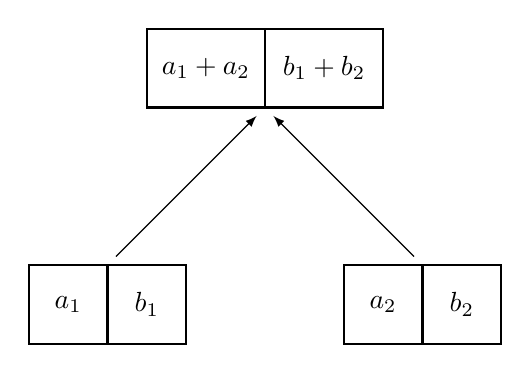
\begin{tikzpicture}

\node (rect) at (1.75,0) [draw,thick,minimum width=1.5cm,minimum height=1cm] {$a_1 + a_2$};
\node (rect) at (3.25,0) [draw,thick,minimum width=1.5cm,minimum height=1cm] {$b_1 + b_2$};


\node (rect) at (0,-3) [draw,thick,minimum width=1cm,minimum height=1cm] {$a_1$};
\node (rect) at (1,-3) [draw,thick,minimum width=1cm,minimum height=1cm] {$b_1$};


\node (rect) at (4,-3) [draw,thick,minimum width=1cm,minimum height=1cm] {$a_2$};
\node (rect) at (5,-3) [draw,thick,minimum width=1cm,minimum height=1cm] {$b_2$};


\draw [arrow]  (0.5,-2.5) to (2.5,-0.5) ;
\draw [arrow]  (4.5,-2.5) to (2.5,-0.5) ;

\end{tikzpicture}
		\caption[MPI\_Reduce]{MPI\_Reduce with MPI\_sum}
		\label{fig:MPIReduce}
	\end{figure}
	\newpage
	\item MPI\_Scatter: This function scatters a sequential array to all processors. Scatter, in this context, means the array is divided into sequential blocks, and every block is sent to another process.
	\begin{figure}[H]
		\centering
		\tikzset{
	main/.style={black, line width=0.4mm, opacity=1},
	second/.style={gray, opacity=5},
	arrow/.style={-latex, shorten >=1ex, shorten <=1ex, bend angle=45}
}
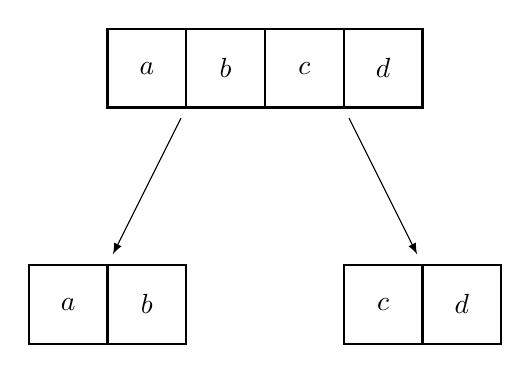
\begin{tikzpicture}
\node (rect) at (1,0) [draw,thick,minimum width=1cm,minimum height=1cm]  {$a$};
\node (rect) at (2,0) [draw,thick,minimum width=1cm,minimum height=1cm]  {$b$};
\node (rect) at (3,0) [draw,thick,minimum width=1cm,minimum height=1cm]  {$c$};
\node (rect) at (4,0) [draw,thick,minimum width=1cm,minimum height=1cm]  {$d$};

\node (rect) at (0,-3) [draw,thick,minimum width=1cm,minimum height=1cm] {$a$};
\node (rect) at (1,-3) [draw,thick,minimum width=1cm,minimum height=1cm] {$b$};

\node (rect) at (4,-3) [draw,thick,minimum width=1cm,minimum height=1cm] {$c$};
\node (rect) at (5,-3) [draw,thick,minimum width=1cm,minimum height=1cm] {$d$};


\draw [arrow]  (1.5,-0.5) to (0.5,-2.5);
\draw [arrow]  (3.5,-0.5) to (4.5,-2.5);

\end{tikzpicture}
		\caption{MPI\_Scatter}
		\label{fig:MPIScatter}
	\end{figure}
	\item MPI\_Gather: This function gathers sequential arrays from all processors. Gather in this context means that there are sequential arrays on every process, and these arrays are gathered to one big sequential array on one processor.
		\begin{figure}[H]
		\centering
		\tikzset{
	main/.style={black, line width=0.4mm, opacity=1},
	second/.style={gray, opacity=5},
	arrow/.style={-latex, shorten >=1ex, shorten <=1ex, bend angle=45}
}
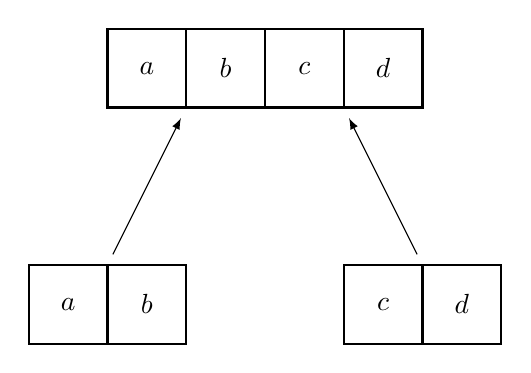
\begin{tikzpicture}
\node (rect) at (1,0) [draw,thick,minimum width=1cm,minimum height=1cm]  {$a$};
\node (rect) at (2,0) [draw,thick,minimum width=1cm,minimum height=1cm]  {$b$};
\node (rect) at (3,0) [draw,thick,minimum width=1cm,minimum height=1cm]  {$c$};
\node (rect) at (4,0) [draw,thick,minimum width=1cm,minimum height=1cm]  {$d$};

\node (rect) at (0,-3) [draw,thick,minimum width=1cm,minimum height=1cm] {$a$};
\node (rect) at (1,-3) [draw,thick,minimum width=1cm,minimum height=1cm] {$b$};

\node (rect) at (4,-3) [draw,thick,minimum width=1cm,minimum height=1cm] {$c$};
\node (rect) at (5,-3) [draw,thick,minimum width=1cm,minimum height=1cm] {$d$};


\draw [arrow]  (0.5,-2.5) to (1.5,-0.5) ;
\draw [arrow]  (4.5,-2.5) to (3.5,-0.5) ;

\end{tikzpicture}
		\caption{MPI\_Gather}
		\label{fig:MPIGather}
	\end{figure}
	
\end{itemize}
\newpage
\subsubsection{Scatter and Gather with specified location and size}
MPI\_Scatter and MPI\_Gather divide the array into equally sized blocks. MPI provides functions where the block sizes can be specified. These functions are denoted with a v at the end, MPI\_Scatterv and MPI\_Gatherv. The array sizes are defined using two additional arrays that have to be passed to the functions. The fist array is called \textit{sendcount} and contains the block sizes. The second array is called \textit{displacement} and contains the starting positions of the blocks. 
	\begin{figure}[H]
	\centering
	\tikzset{
	main/.style={black, line width=0.4mm, opacity=1},
	second/.style={gray, opacity=5},
	arrow/.style={-latex, shorten >=1ex, shorten <=1ex, bend angle=45}
}
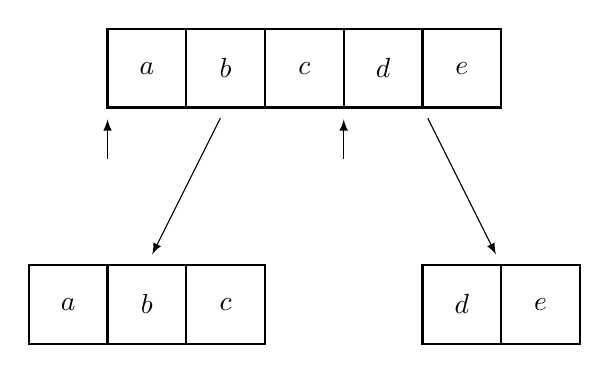
\begin{tikzpicture}
\node (rect) at (1,0) [draw,thick,minimum width=1cm,minimum height=1cm]  {$a$};
\node (rect) at (2,0) [draw,thick,minimum width=1cm,minimum height=1cm]  {$b$};
\node (rect) at (3,0) [draw,thick,minimum width=1cm,minimum height=1cm]  {$c$};
\node (rect) at (4,0) [draw,thick,minimum width=1cm,minimum height=1cm]  {$d$};
\node (rect) at (5,0) [draw,thick,minimum width=1cm,minimum height=1cm]  {$e$};

\node (rect) at (0,-3) [draw,thick,minimum width=1cm,minimum height=1cm] {$a$};
\node (rect) at (1,-3) [draw,thick,minimum width=1cm,minimum height=1cm] {$b$};
\node (rect) at (2,-3) [draw,thick,minimum width=1cm,minimum height=1cm] {$c$};

\node (rect) at (5,-3) [draw,thick,minimum width=1cm,minimum height=1cm] {$d$};
\node (rect) at (6,-3) [draw,thick,minimum width=1cm,minimum height=1cm] {$e$};


\draw [arrow]  (2,-0.5) to (1,-2.5);
\draw [arrow]  (4.5,-0.5) to (5.5,-2.5);

\draw [arrow]  (.5, -1.3) to (.5, -0.5);
\draw [arrow]  (3.5, -1.3) to (3.5, -0.5);
\end{tikzpicture}
	\caption[MPI\_Scatterv]{MPI\_Scatterv sendcount $ = [3,2]$, displacement  $= [0,3]$}
	\label{fig:MPIScatterv}
\end{figure}

\subsubsection{Non-blocking communication with MPI}
The described functions are using blocking communication.
Blocking communication means that the process is blocked until the communication is finished.
During the communication, the computing power of the process is unused.
To prevent this, MPI provides the most communication functions additionally, using non-blocking communication.
These functions are marked with an I at the beginning. For example: MPI\_Scatterv becomes MPI\_Iscatterv.


\subsection{OpenMP - Open Multi-Processing}
OpenMP (Open Multi-Processing) is an application programming interface (API) for multi thread and shared memory programming.
Compared to MPI OpenMP is multi thread. A process can have multiple threads running parallel on the same machine. The threads have access to the virtual memory of their related process.
In this work we make use of OpenMP by using the multi thread property of the Eigen library.

\newpage
\subsection{Eigen}
For the basic linear algebra we use Eigen \cite*{eigenweb}. Eigen is a C++ template library for linear algebra: matrices, vectors, numerical solvers, and related algorithms.\\
Eigen provides the following features that are relevant for the POD:
\begin{itemize}
	\item Data structures for dense vectors and matrices.
	\item Efficient implementations of the general dense matrix-matrix product which can make use of openMP.
	\item Efficient eigenvalue problem solvers.
	\item Efficient singular value decomposition solvers.
\end{itemize}



\newpage

\section{Parallel Algorithm}
\label{sec:paralg}
In this Section we discuss the parallel implementation of the algorithem described in Section \ref{sec:algsimp}.

First the snapshot matrix is partitioned and the partitions are scattered to all processors. $n_p$ is the number of processors.
In some cases the snapshot matrix $W\in\mathbb{R}^{\mathcal{ N } \times n_{train}}$  is already distributed to the processors.

We partition snapshot matrix $\mathcal{W} = [w_0^T w_1^T ... w_{n_p}^T]^T$ in $n_p$ blocks $w_n$. This partitioning is sketched in Figure \ref{fig:Partitioning1}.
The number of rows per block $nr = \mathcal{ N } / n_p$ is calculated by integer dividing the number of rows $\mathcal{ N }$ through the number of processors $n_p$. 
It may be possible that this division generates a rest, which means that not all blocks have the same size.
The remaining rows are obtained using the modulo operation $r = \mathcal{ N } \% n_p$.
To achieve blocks with the fairly same size, we make the first $r$ blocks one row larger.
The dimensions for the blocks $w_n$ are $n\leq r: w_n \in \mathbb{R}^{nr+1 \times n_{train}}$ and  $n > r: w_n \in \mathbb{R}^{nr \times n_{train}}$.

\begin{figure}[H]
	\centering
	\tikzset{
	main/.style={black, line width=0.4mm, opacity=1},
	second/.style={gray, opacity=5},
	arrow/.style={-latex, shorten >=1ex, shorten <=1ex, bend angle=45}
}
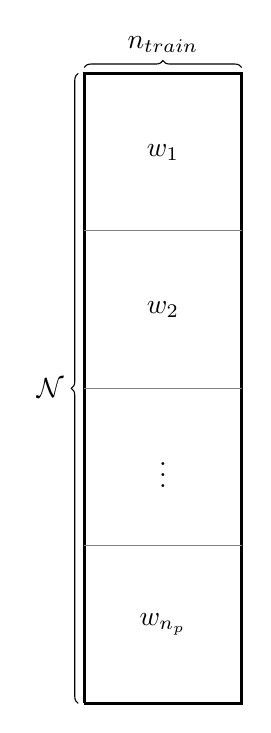
\begin{tikzpicture}
\draw[main] (0,0) -- (2,0) -- (2,8)-- (0,8)-- (0,0);

\draw[second] (0,2) -- (2,2) ;
\draw[second] (0,4) -- (2,4) ;
\draw[second] (0,6) -- (2,6) ;


\draw[decorate, decoration={brace,mirror}, yshift=.5ex]  (2,8) -- node[above=0.4ex] {$n_{train}$}  (0,8);
\draw[decorate, decoration={brace}, xshift=-.5ex]  (0,0) -- node[left=0.4ex] {$\mathcal{ N }$}  (0,8);

\draw (1,7) node {$w_1$};
\draw (1,5) node {$w_2$};
\draw (1,3) node {$\vdots$};
\draw (1,1) node {$w_{n_p}$};


\end{tikzpicture}
	\caption[Partitioning snapshot satrix]{Partitioning of the snapshot matrix $\mathcal{W} \in \mathbb{R}^{\mathcal{ W }\times n_{train}}$ with the parts $w_n$}
	\label{fig:Partitioning1}
\end{figure}

Every block is sent so a processor.
The $n$-th block $w_n$ is sent to the $n$-th processor.
This is done using the function MPI\_Scatterv.
Then every processor computes a local correlation matrix $c_n = w_n^T w_n$.

The global correlation matrix is obtained by summing up all local correlations matrices.
Summing up matrices is adding the corresponding elements of the matrices.
The function MPI\_Reduce provides this feature.
The function collects data of a sequential array from each processor,  adds the corresponding elements and writes the result in a sequential array on the master process.
This gives us the global correlation matrix $C = \sum_{i=0}^{n_p} c_i$.
We solve the eigenvalue problem of the correlation matrix on the master process $C = VS^2V$ using the SelfAdjointEigenSolver from Eigen.

Then the eigenvalues are truncated and the matrix
$$vs = VS^{-\frac{1}{2}}$$
is computed as described in Section \ref{sec:algsimp}.
This matrix is sent to all processors using the function  MPI\_Bcast.
Every processor multiplies the matrix $vs$ on his local copy of the snapshot matrix to obtain the local POD vectors
$u_n = w_n \cdot vs$.

The local POD vectors $u_n$ are gathered to get the global POD vectors in the matrix $U = [u_0^T u_1^T ... u_{n_p}^T]^T$.
This gathering is done by using the function MPI\_Gatherv.
A summary of the implementation is presented in Algorithm \ref{alg:PPOD}.

\begin{algorithm}[H]
	\caption{Pseudocode parallel POD}
	\begin{algorithmic}[1]
		\Function {POD}{$W$}
			\State MPI\_Scatterv( $W$ to $w_n$)
			\State Eigen matrix-matrix product $c_n = w_n^T\cdot w_n$ 
			\State MPI\_Reduce($c_n$, MPI\_sum) $C = \sum_{i=0}^{n_p} c_i$ 
			\If{masterProcess}
				\State Solve EVP $C = VSV^T$ using Eigen
				\State Truncation
				\State $vs = VS^{-\frac{1}{2}}$
			\EndIf
			\State MPI\_Bcast( $vs$ )
			\State Eigen matrix-matrix product $u_n = w_n\cdot vs$
			\State MPI\_Gatherv( $u_n$ in $U$ )
			\State Return $U$
		\EndFunction
	\end{algorithmic}
	\label{alg:PPOD}
\end{algorithm}

\newpage
\subsection{Non-blocking communication}
\label{sec:nonBlockComm}
In this Section we present an extension of the previous algorithm.
We are sending a lot of data because $\mathcal{ N }$ is very big. This leads to a long processor time.
During the communication the processor is idle.
We want to use this idle time by overlapping the communication and the calculations.

MPI provides for all communication functions additionally a non-blocking version.  
These non-blocking versions are marked with a capital I.
MPI\_Scatter becomes MPI\_Iscatter and MPI\_Gather becomes MPI\_Igather.
Non-blocking means that these functions start the communication in the background, so the process is able to continue working and is not blocked by the communication. The only thing we have to make sure, is that we do not use the communication buffer until the communication is finished.

In Algorithm \ref{alg:PPOD} the operations in line 2 and 3 and in line 11 and 12  can be overlapped, using the non-blocking MPI\_Iscatter  MPI\_Igather functions.
We start with the lines 2 and 3.

We use the same partitioning of the snapshot matrix as in the Section before and divide every block additionally in sub-blocks.
We overlap the sending of a matrix sub-block and the computation of the correlation matrix.
In Figure \ref{fig:Bild1} we sketch the partitioning and how the blocks are distributed to the processors. 
The snapshot matrix is stored row major, so it is no problem to block it again row wise.
We call these new blocks sub-blocks.
A sub-block is defined as a compact set of rows. The sub-block size $bs$ is defined as the number of rows of a sub-block.

A block is blocked in the sub-blocks $ w_n = [{w_n^{(1)}}^T, {w_n^{(2)}}^T, ..., {w_n^{(nofbs)}}^T]^T $, where $nofbs$ is the number of sub-blocks.

\begin{figure}[H]
	\centering
	\tikzset{
	main/.style={black, line width=0.4mm, opacity=1},
	second/.style={gray, opacity=5},
	arrow/.style={-latex, shorten >=1ex, shorten <=1ex, bend angle=45}
}
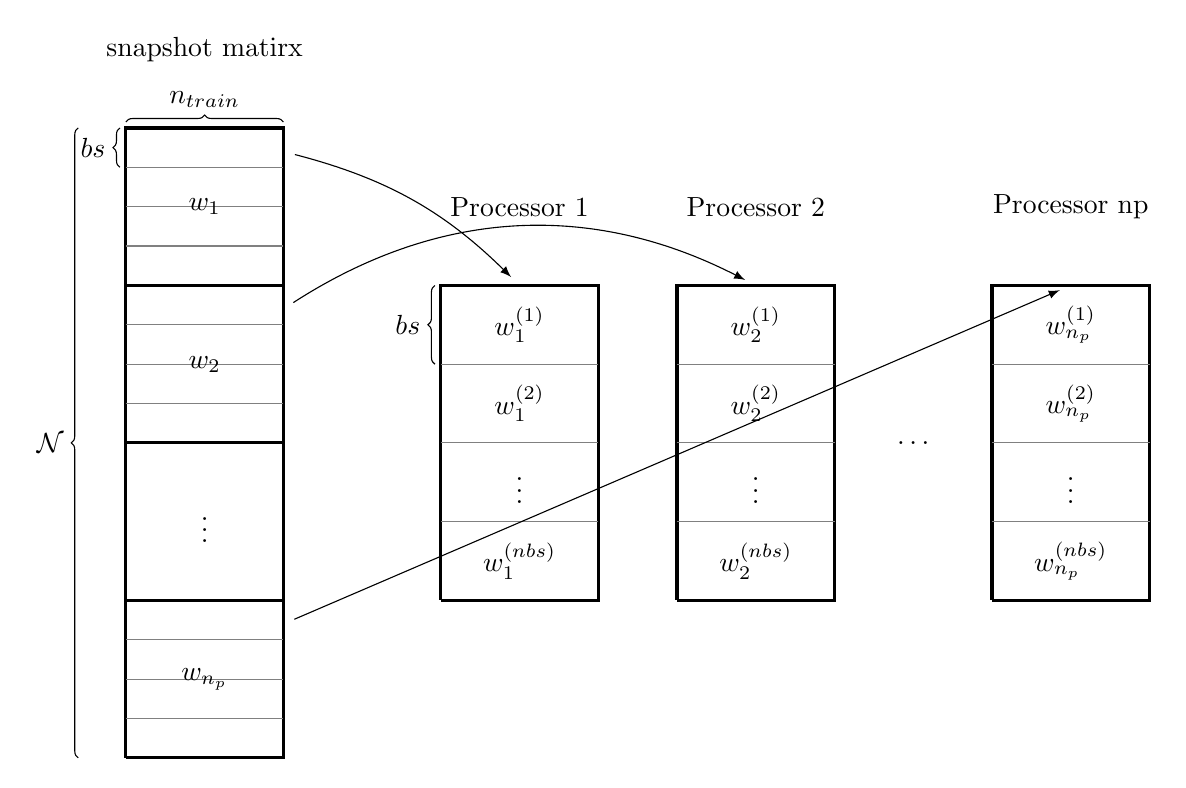
\begin{tikzpicture}
%% Snapshot Matrix
\draw (1,9) node {snapshot matirx};
\draw[main] (0,0) -- (2,0) -- (2,8)-- (0,8)-- (0,0);
\draw[main] (0,2) -- (2,2) ;
\draw[main] (0,4) -- (2,4) ;
\draw[main] (0,6) -- (2,6) ;

\draw[second] (0,7.5) -- (2,7.5) ;
\draw[second] (0,7) -- (2,7) ;
\draw[second] (0,6.5) -- (2,6.5) ;

\draw[second] (0,5.5) -- (2,5.5) ;
\draw[second] (0,5) -- (2,5) ;
\draw[second] (0,4.5) -- (2,4.5) ;

\draw[second] (0,1.5) -- (2,1.5) ;
\draw[second] (0,1) -- (2,1) ;
\draw[second] (0,.5) -- (2,.5) ;

\draw[decorate, decoration={brace,mirror}, yshift=.5ex]  (2,8) -- node[above=0.4ex] {$n_{train}$}  (0,8);
\draw[decorate, decoration={brace}, xshift=-4ex]  (0,0) -- node[left=0.4ex] {$\mathcal{ N }$}  (0,8);
\draw[decorate, decoration={brace}, xshift=-.5ex]  (0,7.5) -- node[left=0.4ex] {$bs$}  (0,8);

\draw (1,7) node {$w_1$};
\draw (1,5) node {$w_2$};
\draw (1,3) node {$\vdots$};
\draw (1,1) node {$w_{n_p}$};

%% prozessor1 Matrix
\draw (5,7) node {Processor 1};
\draw[main] (4,2) -- (6,2) -- (6,6)-- (4,6)-- (4,2);
\draw[second] (4,3) -- (6,3) ;
\draw[second] (4,4) -- (6,4) ;
\draw[second] (4,5) -- (6,5) ;

\draw (5,5.5) node {$w_1^{(1)}$};
\draw (5,4.5) node {$w_1^{(2)}$};
\draw (5,3.5) node {$\vdots$};
\draw (5,2.5) node {$w_{1}^{(nbs)}$};

\draw[decorate, decoration={brace}, xshift=-.5ex]  (4,5) -- node[left=0.4ex] {$bs$}  (4,6);

%% prozessor2 Matrix
\draw (8,7) node {Processor 2};
\draw[main] (7,2) -- (9,2) -- (9,6)-- (7,6)-- (7,2);
\draw[second] (7,3) -- (9,3) ;
\draw[second] (7,4) -- (9,4) ;
\draw[second] (7,5) -- (9,5) ;

\draw (8,5.5) node {$w_2^{(1)}$};
\draw (8,4.5) node {$w_2^{(2)}$};
\draw (8,3.5) node {$\vdots$};
\draw (8,2.5) node {$w_{2}^{(nbs)}$};

%% Dots
\draw (10,4) node {$\dots$};

%% prozessor np Matrix
\draw (12,7) node {Processor np};
\draw[main] (11,2) -- (13,2) -- (13,6)-- (11,6)-- (11,2);
\draw[gray] (11,3) -- (13,3) ;
\draw[gray] (11,4) -- (13,4) ;
\draw[gray] (11,5) -- (13,5) ;

\draw (12,5.5) node {$w_{n_p}^{(1)}$};
\draw (12,4.5) node {$w_{n_p}^{(2)}$};
\draw (12,3.5) node {$\vdots$};
\draw (12,2.5) node {$w_{n_p}^{(nbs)}$};

%% Pfeile
\draw [arrow, bend angle=15, bend left]  (2,7.7) to (5,6);
\draw [arrow, bend angle=30, bend left]  (2,5.7) to (8,6);

\draw [arrow, ]  (2,1.7) to (12,6);


\end{tikzpicture}
	\caption[Partitioning snapshot matrix]{Partitioning of the snapshot matrix for non-blocking communication}
	\label{fig:Bild1}
\end{figure}

The overlapping using non-blocking communication for the lines 2 and 3 of Algorithm \ref{alg:PPOD} is presented in Algorithm \ref{alg:PPODnBlockComm}.

We begin by sending the first sub-block of every block to the corresponding processor of the block.
We do this using MPI\_Iscatterv.
It does not matter if the first sub-blocks are sent in a blocking or a non-blocking way, becaus we can't start computing until the first communication is finished. 
After the first sub-blocks are sent to the processors, the overlapping part starts.
The next sub-blocks are sent in a non-blocking way (see Algorithm \ref{alg:PPODnBlockComm} line 3).
Next we compute correlation matrix of the previous block.
We are now communicating and sending at the same time.
This is done for all sub-blocks.
When all blocks are sent, the last block is computed.
This last computation is not overlapped, because the communication is already finished (see Algorithm \ref{alg:PPODnBlockComm} line 8).

The MPI\_Wait functions in line 4 and 7 of Algorithm \ref{alg:PPODnBlockComm} make sure that we do not access memory, if the communication is not yet finished.

\begin{algorithm}[H]
\caption{Pseudocode overlapping communication}
\begin{algorithmic}[1]
\State MPI\_IScatterV ($w_.^{(1)}$)
\For{$ i = 2:nbs $}
	\State MPI\_IScatterV ($w_.^{(i)}$)
	\State MPI\_Wait(i-1)
	\State Eigen matrix-matrix product $c_n = c_n + {w_n^{(i-1)}}^T\cdot w_n^{(i-1)}$
\EndFor
\State MPI\_Wait(nbs)
\State Eigen matrix-matrix product $c_n = c_n + {w_n^{(nbs)}}^T\cdot w_n^{(nbs)}$
\end{algorithmic}
\label{alg:PPODnBlockComm}
\end{algorithm}

We can use the same overlapping principle from Algorithm \ref{alg:PPODnBlockComm} for the overlapping of lines 11 and 12 in Algorithm \ref{alg:PPOD}.
But in this case it is much simpler.
All the required data for the computation is  already available.
We can compute a block, start to send this block and continue with the same procedure for the next block. We do not have to wait for the communication to be finished while computing.



\subsection{Hybrid approach}
\label{sec:hybimlementaion}
In Section \ref{sec:Benchmarks} we will see that we spend a lot of time by waiting for the communication to be finished,
especially increasing the number of processes because the many global communications can overload the distributed architecture.
We want to reduce the waiting time by reducing the number of communications.
Especially in a pure MPI implementation, every communication on the same note is a copy operation in the RAM.

The idea of the hybrid implementation is to use one MPI process for every processor in the cluster and make this MPI process able to use all cores of the processor using OpenMP.
With this approach, we make use of the shared memory property of OpenMP and get rid of the MPI communications inside a single node.
We only use MPI for the communication between the different processors where communication is necessary anyway.

For the hybrid implementation we use the code described in Algorithm \ref{alg:PPOD},
which brings the advantage that we do not need to change the code.
We use the Eigen library for the matrix-matrix multiplications, and Eigen supports OpenMP.
We have to make sure that we compile the program with OpenMP enabled.
















